\documentclass[journal]{IEEEtran}

\usepackage{cite}
\usepackage{amsmath,amssymb,amsfonts}
\usepackage{graphicx}
\usepackage{tikz}
\usetikzlibrary{arrows.meta,positioning,calc}
\usepackage{algorithm}
\usepackage{algpseudocode}
\usepackage{url}
\usepackage{textcomp}
\usepackage{bm}
\usepackage{multirow}
\usepackage{xcolor}
\usepackage{dblfloatfix}
\usepackage{float}
\usepackage{placeins}
\newcommand{\TBD}[1]{\textcolor{red}{[TBD: #1]}}
\setlength{\textfloatsep}{4pt plus 1pt minus 2pt}
\setlength{\floatsep}{6pt plus 1pt minus 2pt}
\setlength{\intextsep}{6pt plus 1pt minus 2pt}
\setlength{\dbltextfloatsep}{5pt plus 1pt minus 2pt}
\setlength{\dblfloatsep}{6pt plus 1pt minus 2pt}
\setlength{\abovecaptionskip}{3pt}
\setlength{\belowcaptionskip}{0pt}
% Allow two double-column floats at page top (settings+arms)
\setcounter{dbltopnumber}{2}
\renewcommand{\dbltopfraction}{0.9}


\hyphenation{Aqua-Sim under-water event-triggered Bellhop DA-HELLO DA-HELLO LQARP}

\begin{document}

\title{DA-HELLO: State-Carrier-Dependent HELLO Scheduling for
Q-Learning Routing in Underwater Sensor Networks}

% IEEE IoT-J author block. First author: Xuefei Ma.
% Corresponding author: [AUTHOR].
\author{Xuefei~Ma,
        Ghulam~Ali,
        Zhongwei~Shen,
        Insha~Hassan,
        Muhammad~Aon,
        Qingling~Liu,
        Haifeng~Zhu,
        and~Ying~Cui%
\thanks{Xuefei Ma, Zhongwei Shen, Qingling Liu, Haifeng Zhu, and Ying Cui
are with Harbin Engineering University, Harbin 150001, China
(e-mail: maxuefei@hrbeu.edu.cn; shenzhongwei@hrbeu.edu.cn;
liuqingling@hrbeu.edu.cn; zhuhaifeng@hrbeu.edu.cn;
cuiying@hrbeu.edu.cn).}%
\thanks{[AUTHOR] is with \TBD{affiliation: department, institution, city, postcode, country; ORCID 0000-0000-0000-0000} (e-mail: \TBD{institutional e-mail, or confirm [author].cs@gmail.com}). Corresponding author: [AUTHOR].}%
\thanks{Insha Hassan is with \TBD{affiliation; ORCID} (e-mail: inshahassan45@gmail.com).}%
\thanks{Muhammad Aon is with \TBD{affiliation; ORCID} (e-mail: muhammadaoncs29@gmail.com).}}


\markboth{IEEE Internet of Things Journal}%
{Ma \MakeLowercase{\textit{et al.}}: Decision-Aware HELLO Scheduling for Mobile UWSNs}

\maketitle

% IEEE IoT-J: one paragraph, ~150--250 words, no citations, no displayed math.
\begin{abstract}
Q-learning routers for underwater sensor networks rank forwarders using held neighbour state, yet the cost of keeping that state current depends on how the state travels. We study this dependence with DA-HELLO, a configurable HELLO scheduler for a host router. A node sends a HELLO when it first decodes a never-recorded sender, when its candidate membership or void status changes, and, optionally, on a slow refresh; a local score-change test is also included. We evaluate it on two Q-learning routers, MARV and QELAR, each with state carried in data headers and in a constructed HELLO-only variant, in static, drifting, and node-loss scenarios. Comparisons are paired over 40 seeds, statements and margins were fixed before the runs, and idle listening is counted in energy. When state travels only in HELLOs, DA-HELLO delivers 2.1 to 3.0 percentage points more than a jittered 120~s periodic schedule on MARV, with 43 to 53\% fewer control bytes and 8 to 10\% lower energy per bit. On QELAR it uses 45 to 52\% fewer bytes and gains 5.0 points in the static scenario, but is 2.2 and 1.7 points lower in the drifting ones, so non-inferiority at 3 points is not shown. When state is carried in data headers, DA-HELLO matches sending no HELLOs, whereas periodic and Trickle schedules lose delivery. The score-change test shows no demonstrated benefit. The configuration differs by host class, and the results come from simulation of two re-implemented routers.
\end{abstract}

\begin{IEEEkeywords}
HELLO scheduling, neighbour-state maintenance, Q-learning routing, state carriage, underwater acoustic sensor networks.
\end{IEEEkeywords}

\section{Introduction}
\label{sec:intro}
\IEEEPARstart{T}{he} Internet of Underwater Things (IoUT) links sensors, vehicles, and gateways into acoustic multi-hop meshes for environmental observation, resource exploration, and maritime awareness \cite{gupta2024uwsn,gola2023taxonomy,saleem2024ai,jiang2023orsurvey}. Acoustic links offer little bandwidth, long propagation delay, and a time-varying multipath channel \cite{gupta2024uwsn,saleem2024ai,zhu2024trustcomst}, and nodes drift with currents or are carried by vehicles, so a node's neighbourhood keeps changing \cite{gola2023taxonomy,wang2024lgdqn,liu2025mdqn,lu2025wper}. Reinforcement-learning routers have become a common response: each node learns a forwarding policy from the state of its neighbours, such as value estimates, residual energy, depth, and link quality \cite{hu2010qelar,zhang2025saqr,wang2024marv,liu2024clorP,liu2026lqarp}.

Such a router acts on \emph{held} neighbour state, not on the current state of the network, and the way that state reaches the receiver differs between routers. In some, it travels in data headers, so a node that forwards traffic advertises itself at no extra cost, while a node off the forwarding paths advertises nothing. In others, it travels only in HELLO or beacon frames, and some use both (Section~II). The two cases pose different maintenance problems. If state is carried in headers, an additional HELLO may add little. If it is carried only in HELLOs, a missing or old record can make a candidate invisible or wrongly ranked, and the packet is delayed, detoured, or lost. In both cases, every HELLO costs scarce acoustic airtime and energy, including idle listening and the preamble of a short frame.

The literature handles when to re-advertise in three ways: a fixed timer, a timer adapted to mobility \cite{li2025qlar,chen2013apu,zhu2021mobnd}, or a trigger on a void or topology change \cite{ghoreyshi2017void,li2023lrnmp}. Receive-driven replies to a newly overheard neighbour are known from adaptive beaconing in ad hoc networks \cite{chen2013apu}, and void-status beacons from void-handling protocols \cite{ghoreyshi2017void}. What remains open for underwater Q-learning routers is an evaluation that holds the routing logic fixed and varies only the maintenance policy across routers whose state travels in different ways. Most underwater studies also assert that control overhead is negligible without measuring it \cite{zhu2022roeva,zhao2023mlrs,guan2019dvor}, and most energy results leave idle listening out \cite{zhu2022roeva,zhao2023mlrs,li2023lrnmp}.

We address this with DA-HELLO, a configurable HELLO scheduler that sits beside a host router and needs only the host's neighbour query and broadcast primitive. A node sends a HELLO on a first decode of a never-recorded sender, on a change of candidate membership or void status, and, optionally, on a slow refresh; a local score-change test is also included. We evaluate it on two Q-learning routers, MARV and QELAR, and treat LQARP and SAQR as pilot hosts. Our contributions are:
\begin{enumerate}
\item \textbf{Problem.} We formulate neighbour-state maintenance for Q-learning routers as a choice that depends on how state reaches the receiver, in data headers or only in HELLOs, and pose it as minimising control overhead under a bound on the loss of delivery ratio. Without HELLOs, a HELLO-only host collapses to a delivery ratio of 0.06 to 0.18, whereas on header hosts periodic and Trickle HELLOs reduce delivery.
\item \textbf{Method.} DA-HELLO is a configurable scheduler that needs only the host's neighbour query and broadcast primitive. It sends on the first decode of a never-recorded sender, on a change of candidate membership or void status, and optionally on a slow refresh; a local score-change test is also included. We state the evaluated semantics exactly and do not claim that each HELLO is necessary for a receiver's decision.
\item \textbf{Evaluation.} Statements, margins, and seeds were fixed before the runs; comparisons are paired over 40 seeds on MARV and QELAR in header and HELLO-only form, and energy includes idle listening. On HELLO-only MARV, DA-HELLO delivers 2.1 to 3.0 percentage points more than a jittered 120\,s periodic HELLO with 43 to 53\% fewer control bytes and 8 to 10\% less energy per bit. On HELLO-only QELAR it uses 45 to 52\% fewer bytes and gains 5.0 points in the static scenario, but is 2.2 and 1.7 points lower in the drifting ones, so non-inferiority at 3 points is not shown. On header hosts it matches sending no HELLOs. The slow refresh carries delivery on HELLO-only hosts, first-contact replies harm header QELAR, and the score-change test has no demonstrated benefit. Limits of the simulation record are disclosed.
\end{enumerate}
The rest of the article is organised as follows. Section~II reviews related work and the gap. Section~III gives the preliminaries. Section~IV defines the problem and the design. Section~V presents the simulation settings and results, and Section~VI concludes.

\section{Related Work}
\label{sec:related}

This section reviews the literature with a focus on how a node learns
the state of its neighbors and what determines when it re-advertises its
own.
Table~\ref{tab:related} summarizes this for the learning-based UWSN
routers closest to our setting; the remaining subsections cover adaptive
HELLO schemes in Q-learning routers for other mobile networks,
change-driven control messages in ad hoc routing and vehicular
standards, adaptive beaconing and Trickle, and the
estimation and information-freshness literature.

\begin{table*}[t]
\centering
\caption{How learning-based UWSN routers keep neighbor state current
(``n.p.''~=~not published). Last row: DA-HELLO.}
\label{tab:related}
\scriptsize
\setlength{\tabcolsep}{3pt}
\begin{tabular}{@{}l l p{4.0cm} p{3.2cm} p{4.0cm}@{}}
\hline
Protocol & Learning & How neighbor state is disseminated & Control-message interval & Rule for re-advertising \\
\hline
QELAR \cite{hu2010qelar} & Q-learning (model-based) & Carried in data packets & none & Data-driven; no control message \\
CARMA \cite{divalerio2019carma} & Distributed RL & Header fields and overhearing; 6-byte HELLO for discovery & n.p. & Data-driven \\
DROR \cite{wang2023rldepth} & Q-learning + opportunistic & Header fields; sink broadcast on delivery & none & Data-driven \\
SAQR \cite{zhang2025saqr} & Q-learning & Carried in data packets & none & Data-driven \\
Chang \emph{et~al.} \cite{chang2019passive} & RL & Beacon from every node & One per time slot (slot length n.p.) & Fixed timer \\
MARV \cite{wang2024marv} & Multi-agent RL & Header fields plus a periodic control packet & n.p. & Fixed timer \\
CLORP \cite{liu2024clorP} & Multi-agent RL & HELLO message & n.p. & Fixed timer \\
QLAR \cite{li2025qlar} & Q-learning + EKF & Periodic HELLO with position, velocity, and $V$-value & $\tau\min_j T_{\mathrm{LET}}$, $\tau=0.3$ & Timer scaled by predicted link-expiration time under a fixed-range model \\
LQARP \cite{liu2026lqarp} & Q-learning & Header fields ($V$-value, neighbor count); position and energy from one initialization broadcast & none & Data-driven \\
\hline
DA-HELLO (this work) & Q-learning hosts (host-parametric) & HELLO on demand; one broadcast at first contact & Event-driven & Change could alter a neighbor's candidate set or order \\
\hline
\end{tabular}

\end{table*}

\subsection{Learning-Based UWSN Routing and Neighbor-State Maintenance}
Reinforcement-learning routers for underwater networks differ in their
learning rule, ranging from tabular Q-learning with an energy-aware
reward \cite{hu2010qelar} to channel-aware distributed learning
\cite{divalerio2019carma}, service-aware rewards \cite{zhang2025saqr},
void recovery \cite{wang2023rldepth}, multi-agent formulations
\cite{wang2024marv,liu2024clorP}, and rewards built on multipath-aware
link quality \cite{liu2026lqarp}.
They share one requirement: a forwarder needs its neighbors' values
(value estimates, residual energy, depth, or link quality) at decision
time.
The protocols meet it in three ways.

The first is to carry the state in data packets and learn it by
overhearing, as in QELAR, CARMA, DROR, SAQR, and LQARP.
This costs no control traffic, but a node that is not on a forwarding
path advertises nothing.
MARV makes the point explicit: besides the header fields, each node
broadcasts a control packet ``periodically'' so that neighbors learn its
state ``even if they do not have packets to forward''
\cite{wang2024marv}.
The second is a timer.
Chang \emph{et~al.} have every node beacon at the start of each time
slot \cite{chang2019passive}; MARV and CLORP likewise rely on a
periodic control message \cite{wang2024marv,liu2024clorP}.
In these designs the interval is a fixed constant, and in several of
them it is not reported
\cite{chang2019passive,wang2024marv,liu2024clorP}.
Nothing links it to how quickly the advertised state is changing.

The third adapts the timer.
QLAR predicts neighbor positions and velocities with an extended Kalman
filter and sets the HELLO interval to a fraction $\tau$ of the shortest
predicted link-expiration time among neighbors \cite{li2025qlar}.
It is the closest UWSN precedent to our work, and we run its
link-expiration-scaled interval as a baseline (Section~\ref{sec:eval}).
Its connectivity model is a fixed communication range, so link expiry
is a purely geometric event, and it remains a timer rather than a test
of whether the advertised change matters to any neighbor's decision.

Mobility enters the UWSN literature in other ways as well.
Chang \emph{et~al.} model passively drifting sensors but keep the
per-slot beacon \cite{chang2019passive}; cooperative multi-AUV
collection plans vehicle paths with deep Q-learning
\cite{wang2024lgdqn,liu2025mdqn,lu2025wper}; an AUV can be dispatched
to repair isolated sub-networks \cite{nandyala2025isolated};
acoustic--radio meshes switch media opportunistically
\cite{jiang2023hybrid}; routes, power, and link schedules have been
optimized jointly \cite{yuan2024multiobj,yuan2024crosslayer}; and
spatial-temporal graphs record neighbor relations over periodic
intervals for multi-UUV routing \cite{xu2025stgr}.
In these designs motion affects where a vehicle goes or which medium is
used; none uses it to decide when a neighbor should be told.

\subsection{Adaptive HELLO Intervals in Q-Learning and Ad Hoc Routing}
Outside UWSNs, several Q-learning FANET/MANET routers adapt the HELLO
period to speed, neighbor churn, or predicted link lifetime
\cite{liu2020qmr,wei2023qfagr,cui2022tarraq,mahmud2019eehello,han2013hello}.
These schemes set \emph{how often} to advertise from kinematics or
topology change rates; they do not test whether a given attribute change
would alter a learned ranking at a neighbor.
Therefore, rate adaptation alone does not address decision relevance for
Q-learning hosts.

\subsection{Change-Driven Control Messages}
Triggered updates appear in classical ad hoc routing and neighbor
discovery: DSDV triggered updates, TBRPF next-hop-relevant reporting,
NHDP responsive HELLOs, and ETSI CAM rules keyed on kinematics
\cite{perkins1994dsdv,rfc3684,rfc6130,etsi302637}.
The common pattern is to advertise when a link, metric, or trajectory
changes beyond a threshold.
However, the trigger is defined on topology or kinematics rather than on
whether a \emph{learned} score would change a neighbor's next-hop choice.
Therefore, a decision-relevance test for Q-learning hosts remains open.

\subsection{Adaptive Beaconing and Trickle}
Terrestrial networks adapt the beacon rate to speed or neighbor turnover
\cite{ingelrest2007tap,sadiq2013beaconing}.
Trickle doubles its interval while neighbors are consistent and resets on
inconsistency \cite{levis2004trickle,rfc6206}; RPL applies it to routing
control and resets on routing-state inconsistency \cite{rfc6550}.
These schemes answer \emph{how often} to beacon given mobility or churn,
not whether a given change would alter a learned candidate order.
We therefore use periodic timers and a tuned Trickle as baselines.

\subsection{Event-Triggered Estimation and the Value of Updates}
Event-triggered estimation transmits an update when a prediction residual
or innovation exceeds a threshold
\cite{priel2023consensus,sebastian2024eco,deng2023auto,deng2024lcsys,zhong2024tsp}.
Li \emph{et~al.} use media-specific triggers for a hybrid underwater
network \cite{li2026dse}; Kalman and Markov models have been compared for
predicting acoustic SNR from traces \cite{busacca2024snr}.
In all of these works the trigger protects an estimation error.
Age-of-information scheduling instead asks how often a source should
update so that the receiver's information stays fresh
\cite{kaul2012aoi,yates2021aoisurvey}; value-of-information and
goal-oriented communication transmit an update only when it matters to
the receiver's goal
\cite{ayan2019voi,kountouris2021semantics,li2024got}.
Our trigger is a concrete instance of this goal-oriented principle in
which the receiver's goal is its next-hop choice; it does not use an
estimation-error trigger.

\subsection{Positioning and Research Gap}
The principle ``advertise only what can change a neighbor's routing
decision'' is therefore not new: it appears in DSDV triggered updates,
TBRPF's next-hop-relevant reporting, NHDP responsive HELLOs, RPL's
inconsistency reset, QFAGR's hole broadcasts, TARRAQ's event-driven
sensing interval, and goal-oriented updating.
On the campaigned hosts, the realized DA-HELLO traffic under locked
configurations is dominated by first-contact replies, membership
(void-status) events, and optional slow refresh rather than by a
continuously firing rank test.
What remains open, and what this paper contributes, is narrower.
First, a formal definition of decision relevance for \emph{learned}
scores: a change is relevant if it alters whether a node is a candidate
of some neighbor or flips the sign of a score gap to a co-candidate
(Section~\ref{sec:prelim}), which no shortest-path or threshold rule
captures for Q-learning hosts.
Second, a local, host-parametric estimator of that test that a sender
can evaluate from the information it is allowed to hold, with the host
entering only through its candidate test and score.
Third, a cross-host evaluation of HELLO scheduling for Q-learning UWSN
routers with different control planes, against tuned adaptive
baselines that include QLAR's link-expiration timer, under one
energy-accounting rule that includes idle listening, and on a shared
acoustic medium with a contention MAC, half-duplex operation, and
heard-only neighbor discovery.

\section{SYSTEM MODEL AND PROBLEM FORMULATION}
\label{sec:prelim}
DA-HELLO acts on neighbour state that a node holds, so this section defines what a node can know and how that state reaches it. It introduces the two state carriers that organise the rest of the paper and contains no parameter values; those are given in Section~\ref{sec:eval}.

\subsection{Network and Mobility}
\label{sec:network}
A set of relays $\mathcal{S}=\{s_1,\dots,s_N\}$ and one fixed sink $s_0$ share an acoustic medium in a three-dimensional volume (Fig.~\ref{fig:network}). Each relay $s_i$ has a position $\mathbf{p}_i(t)$, a depth $z_i(t)$, a residual energy $e_i(t)$, a queue, learning variables, and timers. Sensing nodes generate packets, and every packet is addressed to the sink and relayed hop by hop.

Relays drift with the water. The velocity of relay $s_i$ follows a Gauss--Markov process with memory $\zeta$ around a position-dependent mean flow $\boldsymbol{\mu}(\mathbf{p})$,
\begin{equation}
\mathbf{v}_i(t{+}\Delta)=\zeta\,\mathbf{v}_i(t)+(1-\zeta)\,\boldsymbol{\mu}(\mathbf{p}_i)+\sqrt{1-\zeta^2}\,\boldsymbol{\Sigma}\,\mathbf{w}_i,
\label{eq:gm}
\end{equation}
where $\mathbf{w}_i$ is standard Gaussian noise and $\boldsymbol{\Sigma}$ sets the per-axis deviation. The mean flow models a mesoscale eddy as a counter-clockwise tangential flow around a centre $\mathbf{c}$ with radius $R$ and peak speed $V$,
\begin{equation}
\boldsymbol{\mu}(\mathbf{p})=V\,\min\!\Big(\tfrac{\rho}{R},1\Big)\,\hat{\mathbf{e}}_\theta,\qquad \rho=\|\mathbf{p}_{xy}-\mathbf{c}\|,
\label{eq:eddy}
\end{equation}
so nodes at different radii move differently and links break and form. The sink is stationary. A relay that leaves the volume is removed for the rest of the run. Static scenarios correspond to $V=0$ and $\boldsymbol{\Sigma}=\mathbf{0}$.

\begin{figure}[t]
\centering
% t182: Ali-supplied Fig. 1 (t116 schematic). Do not hand-edit the PDF.
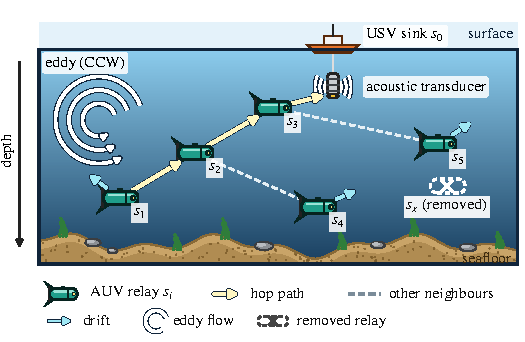
\includegraphics[width=\columnwidth]{fig1_network}

\caption{Network model (side view). Relays drift under an eddy and Gauss--Markov flow, so decodable links form and break; packets are forwarded hop by hop to the fixed sink. A relay that leaves the volume is removed. Each relay forwards using \emph{held} records of its neighbours, whose upkeep is the subject of this work.}
\label{fig:network}
\end{figure}

\subsection{Channel, Frames, and Energy}
\label{sec:channel}
Only the medium evaluates propagation and reception. The signal-to-noise ratio of a frame sent over a distance $d$ is
\begin{equation}
\mathrm{SNR}(d)=\mathrm{SL}-10\kappa\log_{10}d-\alpha(f_c)\,d-N_0,
\label{eq:snr}
\end{equation}
with source level $\mathrm{SL}$, spreading exponent $\kappa$, Thorp absorption $\alpha(f_c)$ at carrier frequency $f_c$, and ambient noise level $N_0$, all in decibels. Frames use non-coherent binary frequency-shift keying, for which the bit error rate is $p_b=\tfrac12\exp(-\gamma_b/2)$ with $\gamma_b=\mathrm{SINR}\cdot B/R_b$, and the frame error rate is $1-(1-p_b)^{\ell_f}$ for a frame of $\ell_f$ bits. Concurrent frames interfere, and a half-duplex node cannot receive while it transmits. A frame of $\ell_f$ bits occupies the channel for
\begin{equation}
T_f=T_{\mathrm{pre}}+\ell_f/R_b,
\label{eq:duration}
\end{equation}
so a short control frame is dominated by its preamble $T_{\mathrm{pre}}$. A node draws the powers $P_{\mathrm{tx}}$, $P_{\mathrm{rx}}$, and $P_{\mathrm{idle}}$ in the transmit, receive, and idle-listening states, and it listens continuously. A control frame therefore costs $T_f(P_{\mathrm{tx}}-P_{\mathrm{idle}})$ at the sender and $T_f(P_{\mathrm{rx}}-P_{\mathrm{idle}})$ at each receiver above the idle baseline, and it also consumes airtime that data frames could use.

\subsection{Locally Available Information}
\label{sec:info}
A node $s_i$ learns of a neighbour $s_j$ only by decoding a frame from it. Let $b_{ij}(t)$ be the latest time at which $s_i$ accepted a state-bearing frame from $s_j$, with $b_{ij}=-\infty$ if none. A record is \emph{fresh} when
\begin{equation}
L_{ij}(t)=\mathbf{1}\{b_{ij}(t)>-\infty,\; t-b_{ij}(t)\le T_{\mathrm{nb}}\},
\label{eq:fresh}
\end{equation}
and only fresh records can form candidates. At time $t$, the routing logic and the HELLO policy of $s_i$ may use only: its own state and timers; the fields of frames it has decoded, as written by the sender at transmission start; the received SNR and decode time of those frames; held records built from them, possibly stale; a-priori constants such as the PHY and MAC settings and the fixed sink position; and the outcome of its own transmissions. A node never reads another node's true position, depth, energy, or neighbour set.

\subsection{State Carriers and Host Interface}
\label{sec:carriers}
Each node $s_j$ has an advertised attribute vector $\xi_j(t)$ that its neighbours need, such as a value estimate, residual energy, depth or position, and a void flag. A frame carries a subset of it. We distinguish two \emph{state carriers} (Fig.~\ref{fig:carriers}). In the \emph{header-carried} regime, data frames carry the attributes, so a forwarding node advertises itself at no extra control cost, and a HELLO supplements this for nodes off the forwarding paths. In the \emph{HELLO-only} regime, data frames carry none, and a held record is written only by HELLO or beacon frames. Real protocols may mix the two. In Section~\ref{sec:eval}, the HELLO-only regime is a constructed variant of each host, not a reproduction of a published protocol.

\begin{figure}[t]
\centering
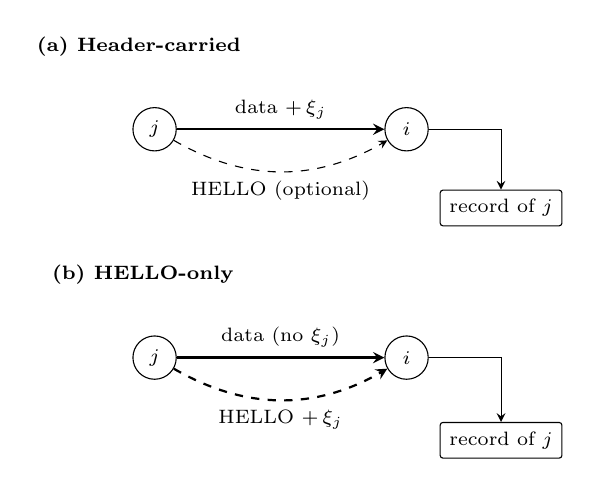
\begin{tikzpicture}[font=\scriptsize,>=stealth,node distance=0.5cm,
 nd/.style={circle,draw,minimum size=0.55cm,inner sep=0pt},
 tb/.style={draw,rounded corners=1pt,minimum width=1.5cm,minimum height=0.45cm,align=center}]
% panel a
\node[font=\scriptsize\bfseries] at (-0.2,2.55) {(a) Header-carried};
\node[nd] (a1) at (0,1.5) {$j$};
\node[nd] (a2) at (3.2,1.5) {$i$};
\draw[->,thick] (a1) -- node[above,pos=.5]{data $+\,\xi_j$} (a2);
\draw[->,dashed] (a1) to[bend right=30] node[below,pos=.5]{HELLO (optional)} (a2);
\node[tb] (ta) at (4.4,0.5) {record of $j$};
\draw[->] (a2) -| (ta);
% panel b
\node[font=\scriptsize\bfseries] at (-0.15,-0.35) {(b) HELLO-only};
\node[nd] (b1) at (0,-1.4) {$j$};
\node[nd] (b2) at (3.2,-1.4) {$i$};
\draw[->,thick] (b1) -- node[above,pos=.5]{data (no $\xi_j$)} (b2);
\draw[->,dashed,thick] (b1) to[bend right=30] node[below]{HELLO $+\,\xi_j$} (b2);
\node[tb] (tb) at (4.4,-2.45) {record of $j$};
\draw[->] (b2) -| (tb);
\end{tikzpicture}

\caption{The two state carriers. (a) Header-carried: a data frame writes the sender's attributes into the receiver's held record; a HELLO is optional. (b) HELLO-only: data frames write nothing, and a record exists only after a HELLO or beacon has been decoded, so maintenance determines whether a neighbour can be ranked at all.}
\label{fig:carriers}
\end{figure}

A host router $h$ is described by an eligible candidate set $\mathcal{I}^h_i(t)$ of node $s_i$, built from fresh records, and a forwarding output $\mathcal{R}_h$ that orders the candidates by a score $\sigma_i(j)$ and selects a next hop. The scheduler of Section~\ref{sec:design} uses the host through three primitives only: the candidate set and held records of the node itself, its own advertised vector, and a broadcast of a control frame. It does not use the host's learning rule. The hosts differ in their eligibility rules: in MARV a candidate has a fresh record, a held depth shallower than the sender, and no excluding void flag, and candidates are ordered by updated Q values; in QELAR a candidate has a fresh record and passes an admission test on its held SNR, without a depth restriction, and the largest stored Q value selects the next hop.

\subsection{Held State and Its Staleness}
\label{sec:stale}
Between two accepted frames from $s_j$, node $s_i$ holds a zero-order copy $\hat{\xi}_{ij}$ of the advertised vector, while the true attributes $\xi_j(t)$ keep evolving with motion, energy use, and learning. The copy is wrong for $s_i$'s purposes only if the error changes what $s_i$ does: whether $s_j$ is a candidate, how it ranks against another candidate, or whether $s_i$ can see $s_j$ at all. A record that is merely old is not necessarily wrong. This distinction, which Section~\ref{sec:problem} formalises, is what separates deciding when to re-advertise from running a timer.

\subsection{Metrics and Accounting}
\label{sec:metrics}
For a run $r$, let $G_r$ be the number of application packets generated in the analysis interval $[t_w,t_g)$ after a warm-up $t_w$, and $D_r$ the number of those packets that reach the sink. The run-level delivery ratio and energy per delivered bit are
\begin{equation}
p_r=\frac{D_r}{G_r},\qquad e_r=\frac{E_r}{\ell\,D_r},
\label{eq:runmetrics}
\end{equation}
where $\ell$ is the data payload length and $E_r$ is the modem energy of all nodes accumulated over $[t_w,t_g+t_d]$, which includes a drain period $t_d$ after the last generation. It covers transmit, receive, and idle-listening states, so idle energy is always counted, and it excludes propulsion and other platform loads. A relay that is removed stops generating packets, but packets it already offered stay in $G_r$. The packet cohort and the energy interval are therefore different intervals, and we do not call either of them ``the window''.

The primary summaries average run-level ratios, $\bar p=\mathbb{E}[p_r]$ and $\bar e=\mathbb{E}[e_r]$, over seeds. They differ from pooled estimates,
\begin{equation}
\hat p_{\mathrm{pool}}=\frac{\sum_r D_r}{\sum_r G_r},\qquad \hat e_{\mathrm{pool}}=\frac{\sum_r E_r}{\ell\sum_r D_r},
\label{eq:pooled}
\end{equation}
and one cannot be reported as the other. When $D_r=0$, $e_r$ is undefined, not zero, and the run's energy still belongs in the pooled numerator. The control overhead is
\begin{equation}
O_{\mathrm{ctrl}}=\frac{1}{t_g}\sum_{f\in\mathcal{F}}\frac{\ell_f}{8},
\label{eq:octrl}
\end{equation}
where $\mathcal{F}$ is the set of HELLO and beacon frames that start in $[0,t_g]$, with $\ell_f$ in bits. It charges the initial announcements and the sink beacon and excludes frames that start during the drain. The control count, the packet cohort, and the energy interval have deliberately different definitions.

\section{Problem Definition and DA-HELLO Design}
\label{sec:design}
A HELLO is useful only if it changes what a receiver does, yet a sender cannot see its receivers' state. This section states that as a scheduling problem and then gives DA-HELLO, a causal heuristic that approximates it from the sender's own history. Only the scheduler is described here; the host routers and the state carriers are those of Section~\ref{sec:prelim}.

\subsection{Problem Definition}
\label{sec:problem}
Let $U_{j,k}\in\{0,1\}$ indicate that node $s_j$ requests a HELLO at decision epoch $k$ of period $\Delta t$. A request can be queued, delayed, or dropped by the MAC, and a transmitted HELLO can collide or fall below the decoding threshold, so a request neither guarantees a transmission nor refreshes any particular receiver. Between frames, every receiver holds a zero-order copy of the advertised vector $\xi_j$, while the true attributes keep evolving.

Not every change matters to a receiver. Let $m_j$ be an advertisement of $s_j$ and $\mathcal{U}_h(X_i^h,m_j,y_{ij})$ the host's processing of its successful reception at $s_i$, where $X^h_i$ holds the held records and learning state and $y_{ij}$ is the reception metadata. For a diagnostic recipient set $\mathcal{C}_j$, define
\begin{multline}
D_j=\mathbf{1}\big\{\exists\, i\in\mathcal{C}_j:\ \mathcal{R}_h(X_i^{h,+};\kappa_i)\neq \mathcal{R}_h(X_i^h(t^-);\kappa_i)\big\},\\
X_i^{h,+}=\mathcal{U}_h\big(X_i^h(t^-),m_j,y_{ij}\big),
\label{eq:relevance}
\end{multline}
that is, the advertisement matters if some receiver's forwarding output $\mathcal{R}_h$ for a packet context $\kappa_i$ would change. Missing and expired records are included in the hypothetical reception, so a first contact is relevant because a node that has never recorded $s_j$ cannot rank it. Candidacy changes and sign changes of the score gap $g_{ijc}=\sigma_i(j)-\sigma_i(c)$ to a co-candidate $s_c$ are the two ways the output can change. $D_j$ is a receiver-specific offline \emph{diagnostic}: it needs the receivers' state, so it cannot be an input to a node, and it was not measured in our campaign. An update can also be useful later when the immediate output is unchanged, and a changed output can be harmful, so $D_j$ does not define an optimal schedule.

Let $B(\pi)$ be the control bytes sent under a HELLO policy $\pi$ and $\mathrm{PDR}(\pi)$ the delivery ratio of a fixed host router. With a reference policy $\pi_{\mathrm{ref}}$ and a non-inferiority margin $\delta_P$, the \emph{host-parametric HELLO scheduling problem} is
\begin{equation}
\min_{\pi}\ \mathbb{E}\,[B(\pi)]\quad\text{s.t.}\quad \mathbb{E}\,[\mathrm{PDR}(\pi)]\ \ge\ \mathbb{E}\,[\mathrm{PDR}(\pi_{\mathrm{ref}})]-\delta_P,
\label{eq:problem}
\end{equation}
over causal policies $U_{j,k}=\pi_j(\mathcal{H}_j(t_k),Z_{j,k})$ that depend only on the node's own history $\mathcal{H}_j$ and local randomness $Z_{j,k}$. The problem involves the host only through the candidate set $\mathcal{I}^h$ and the score $\sigma_i$, not through its learning rule, so any host that exposes them poses the same problem. Energy enters through $B$ and through the delivery count in (\ref{eq:runmetrics}). DA-HELLO is an experimentally assessed heuristic for (\ref{eq:problem}), not an optimiser, and sending a HELLO exactly when $D_j=1$ is not claimed to be optimal. The reference in our primary HELLO-only comparison is the 120\,s periodic policy, not a policy selected for its outcome.

\subsection{Design Overview}
\label{sec:overview}
DA-HELLO follows three principles. It is \emph{host-parametric}: it uses the host only through the candidate set, the score, and a broadcast primitive. It is \emph{causal}: every input is the node's own state, a decoded frame, or a held record. And it works on \emph{requests}: the scheduler decides when to ask for a HELLO, and the MAC decides when, and whether, it is sent. Fig.~\ref{fig:flow} shows the structure. All policies in Section~\ref{sec:eval}, including the no-HELLO arm, start from the same join announcement: each node sends one HELLO after a random delay, and the sink broadcasts a beacon at a fixed period throughout. After joining, DA-HELLO raises a request on four conditions.

\begin{figure*}[t]
\centering
% t183: Ali-supplied Fig. 3 (replaces TikZ fig_flow). Do not hand-edit the PDF.
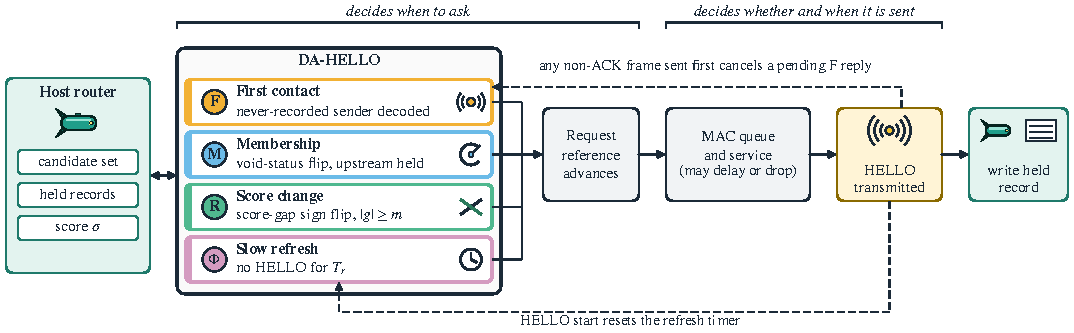
\includegraphics[width=\textwidth]{fig3_flow}

\caption{Structure of DA-HELLO beside a host router. Four conditions on the node's own history raise a request; the request advances a sender reference, passes through the MAC, and a HELLO that is decoded writes the receivers' held records. A pending first-contact reply is cancelled if the node sends any non-ACK frame first.}
\label{fig:flow}
\end{figure*}

\subsection{Trigger Conditions}
\label{sec:policy}
At epoch $k$, a node requests a HELLO if
\begin{equation}
U_{j,k}=\mathbf{1}\{F_j\vee M_{j,k}\vee R_{j,k}\vee \Phi_{j,k}\},
\label{eq:request}
\end{equation}
where the conditions are evaluated in the order $M$, $R$, $\Phi$ and at most one request is raised per epoch. One HELLO serves all pending requests of the node.

\emph{First contact ($F$).} When $s_j$ decodes a frame from a sender $s_x$ that it has never recorded, it schedules a reply after a random delay $u\sim\mathcal{U}[0,u_{\max}]$, with a minimum separation $g_{\min}$ between reply releases. Several discoveries can share one pending reply, and the separation is a release-side limit, not a bound on the spacing of physical transmissions after MAC queueing. The test uses the node's own record of $s_x$ before the frame is written. That record is created by the first decoded state-bearing frame and is never cleared, so ``new'' means never recorded, not recorded and since expired. The reply is cancelled if the node begins any non-ACK transmission before it fires.

\emph{Membership ($M$).} Let $v_j(t)=\mathbf{1}\{\mathcal{I}^h_j(t)=\emptyset\}$ be the void indicator of $s_j$ and $\mathcal{A}_j(t)$ the approximate upstream-interest set formed from its fresh records and held depths. Then
\begin{equation}
M_{j,k}=\mathbf{1}\{v_j(t_k)\neq v_j^{\mathrm{ref}}\ \wedge\ \mathcal{A}_j(t_k)\neq\emptyset\},
\label{eq:membership}
\end{equation}
where $v_j^{\mathrm{ref}}$ is the void status at the last request. This is a void-status heuristic, not a detector for every change in a receiver's candidate set: a receiver that $s_j$ has never heard can be absent from $\mathcal{A}_j$.

\emph{Score change ($R$).} Let $g^{\mathrm{ref}}_{jc}$ and $g^{\mathrm{now}}_{jc}$ be the score gap between $s_j$ and a held co-candidate $s_c$ computed with the score at the last request and with the current score. A non-void node raises
\begin{multline}
R_{j,k}=\mathbf{1}\{v_j(t_k)=0\ \wedge\ t_k\ge\tau_j\ \wedge\\
\exists\, c:\ g^{\mathrm{ref}}_{jc}\,g^{\mathrm{now}}_{jc}<0,\ |g^{\mathrm{now}}_{jc}|\ge m\},
\label{eq:rank}
\end{multline}
with margin $m$ and hold deadline $\tau_j$. A void event resets the interval $I_j$ to $I_{\min}$; each accepted rank event doubles it up to $I_{\max}=I_{\min}2^{d}$ with $d$ doublings and sets $\tau_j=t_k+I_j$. This back-off acts on rank requests only; it is distinct from MAC contention back-off and from Trickle's consistency-based suppression.

\emph{Slow refresh ($\Phi$).} With period $T_r$ and the time $t^{\mathrm{last}}_j$ of the node's last HELLO,
\begin{equation}
\Phi_{j,k}=\mathbf{1}\{T_r<\infty\ \wedge\ t_k-t^{\mathrm{last}}_j\ge T_r\},
\label{eq:refresh}
\end{equation}
and $T_r=\infty$ disables it.

\subsection{Algorithm}
\label{sec:algo}
Algorithm~\ref{alg:da} gives the receive handler and the per-epoch procedure.

\begin{algorithm}[t]
\caption{DA-HELLO at node $s_j$}
\label{alg:da}
\begin{algorithmic}[1]
\Require held records; references $g^{\mathrm{ref}}_{jc}$, $v^{\mathrm{ref}}_j$, $t^{\mathrm{last}}_j$, $\tau_j$; parameters $(m,I_{\min},d,T_r,u_{\max},g_{\min})$
\Statex \textbf{On decode of a frame from $s_x$ (before the record is written):}
\If{$s_x$ never recorded by $s_j$}
  \State schedule or merge a first-contact reply after $u\sim\mathcal{U}[0,u_{\max}]$, not earlier than $g_{\min}$ after the previous reply release
\EndIf
\Statex \textbf{On start of any non-ACK transmission of $s_j$:}
\State cancel the pending first-contact reply
\Statex \textbf{At each epoch $t_k$:}
\State $U\gets 0$
\If{$M_{j,k}=1$}
  \State $U\gets 1$; $I_j\gets I_{\min}$ \Comment{membership}
\ElsIf{$R_{j,k}=1$}
  \State $U\gets 1$; $I_j\gets\min(2I_j,\,I_{\min}2^{d})$; $\tau_j\gets t_k+I_j$ \Comment{score change}
\ElsIf{$\Phi_{j,k}=1$}
  \State $U\gets 1$ \Comment{slow refresh}
\EndIf
\If{$U=1$}
  \State update $g^{\mathrm{ref}}_{jc}$ and $v^{\mathrm{ref}}_j$ from the current state; request a HELLO
\EndIf
\end{algorithmic}
\end{algorithm}

\subsection{Host Instantiation}
\label{sec:hosts}
The score $\sigma$ is host-specific, and each surrogate below is a local approximation of the order that neighbours compute. For MARV it is
\begin{equation}
\sigma^{\mathrm{M}}_j=-w_E\Big(1-\frac{e_j}{E_0}\Big)-w_D\frac{z_j}{R_s}+\gamma(\lambda_1-\lambda_2)V_j,
\label{eq:marv_score}
\end{equation}
with the host's energy and depth weights $w_E,w_D$, normalisation energy $E_0$, range scale $R_s$, and value $V_j$. The current self depth is used in both the reference and the current score, and competitor values come from the node's own held records, with the fixed sink depth taken as an a-priori constant. For QELAR it is
\begin{equation}
\sigma^{\mathrm{Q}}_j=\frac{e_j}{E_0}+c_n\,n_j+\gamma\,V_j,
\label{eq:qelar_score}
\end{equation}
with $n_j$ the size of the candidate set and $V_j$ the node's own value; the peer score uses the held energy of $s_c$ and sets its count and value to zero. This is a heuristic proxy for the stored Q-ordering of neighbours, not an exact reconstruction, and the asymmetric substitution can influence which crossings occur. Because the rank test rests on a surrogate, a rank request is evidence for a trigger condition, not proof that a remote forwarding decision changed. The constants $c_n$ and $\gamma$ are the host's own.

\subsection{Request Semantics of the Evaluated Implementation}
\label{sec:semantics}
Four details matter for reading the results. First, the medium samples the sender's advertised fields into a frame at the start of an actual control transmission, and receivers apply those sampled values after decoding, so a later sender value is never substituted at decode time. Second, the references advance when a request is accepted by the scheduler, before the MAC serves it, so a reference is the last requested value, not necessarily the last transmitted one; MARV also advances its sender reference on a data transmission, including in the HELLO-only variant where receivers ignore the attributes of data frames. Third, the cancellation rule is kind-based: any non-ACK transmission cancels a pending reply, whether or not it carried the fields the reply would have supplied, and in the HELLO-only variants this includes stripped data frames. Fourth, the refresh timer is reset at the start of a HELLO transmission in MARV, but at the request and at control transmissions in QELAR, so a configured $T_r$ is not a bound on the age of a receiver's record. Counters of membership, rank, refresh, and reply-release \emph{requests} are therefore never summed as HELLOs; physical control traffic is counted from the medium's frame-start tally. A stricter field-aware controller would change the policy, and its results would not follow from those reported here.

\subsection{Properties and Scope}
\label{sec:scope}
The per-epoch cost is $O(|\mathcal{N}_j|)$ in the number of held neighbours. Beyond the host primitives of Section~\ref{sec:prelim}, DA-HELLO adds a few scalars of state per node ($g^{\mathrm{ref}}_{jc}$, $v^{\mathrm{ref}}_j$, $t^{\mathrm{last}}_j$, $\tau_j$) and a pending-reply timer. It is host-parametric in the sense that it needs only $\mathcal{I}^h$, $\sigma$, and a broadcast primitive. It is not self-configuring: the parameters differ by host class and state carrier (Section~\ref{sec:eval}).

\section{Simulation Settings and Results}
\label{sec:eval}
We evaluate DA-HELLO on two Q-learning routers, MARV~\cite{wang2024marv} and QELAR~\cite{hu2010qelar}, each in two state-carrier regimes, and report pilot runs on LQARP~\cite{liu2026lqarp} and SAQR~\cite{zhang2025saqr}, which did not qualify as hosts. Statements, margins, arms, and seeds were fixed before the evaluation runs. All numbers below are means over seeds of run-level ratios, with ordinary 95\% Student-$t$ intervals.

\subsection{Simulation Settings}
\label{sec:settings}
Experiments run in ns-3 with an acoustic modem and a shared-medium MAC. Table~\ref{tab:settings} lists the settings, and Fig.~\ref{fig:deploy} shows one placement. A volume of $4000\times4000\times3500$~m holds 149 relays and a stationary sink at the centre of the horizontal plane; positions are drawn uniformly at random per seed. Every relay generates one packet on average every 1200~s, and neighbour records are created only by decoded frames (heard-only discovery) and expire after $T_{\mathrm{nb}}$. Idle listening is charged for the whole run, so every energy figure includes it.

\begin{table*}[!t]
\caption{Simulation Settings (Evaluation Campaigns t103/t109).
Scheduler Parameters Are Those Locked in Section~\ref{sec:arms}.}
\label{tab:settings}
\centering
\scriptsize
\setlength{\tabcolsep}{4pt}
\begin{tabular*}{\textwidth}{@{\extracolsep{\fill}}ll@{\hspace{1.2em}}ll@{}}
\hline
Parameter & Value & Parameter & Value \\
\hline
Volume / $N$ & $4{\times}4{\times}3.5\,\mathrm{km}$ / $149{+}1$
  & Bit rate / HELLO, data / ACK & $5\,\mathrm{kbit/s}$ / $400$ / $64\,\mathrm{bit}$ \\
$P_{\mathrm{tx}}$ / $P_{\mathrm{rx}}$ / $P_{\mathrm{idle}}$
  & $8$ / $1.3$ / $0.285\,\mathrm{W}$
  & MAC / channel / discovery & CS / formula / heard \\
$T_{\mathrm{sim}}$ / warm / drain & $14400$ / $900$ / $300\,\mathrm{s}$
  & Data interval / $T_{\mathrm{nb}}$ / beacon & $1200$ / $3600$ / $60\,\mathrm{s}$ \\
Eddy centre / radius & $(2000,2000)$ / $2828\,\mathrm{m}$
  & Sc.~I / II / GM2 & static / $V{=}0.15$ / $V{=}0.3$ \\
Relay removal (II/GM2) & $22\%$ / $30\%$ (means)
  & Periodic $T$ (jittered) & $\{20{..}120\}$ / $\{60,120\}$ \\
B2* Trickle & $I_{\min}{=}20\,\mathrm{s}$, $8$ dbl., $k{=}5$
  & Eval.\ seeds ($n{=}40$) & $20261801$--$40$ / $20261841$--$80$ \\
Tuning seeds (pilots) & $20261114$--$23$
  & Non-inf.\ margin & $0.5\,\mathrm{pp}$ / $3\,\mathrm{pp}$ (QELAR) \\
\hline
\end{tabular*}
\end{table*}

\begin{table*}[!t]
\caption{HELLO Arms Shared Across Hosts. Only the Scheduler Differs;
Join Announcement and 60~s Sink Beacon Are Common to Every Arm.}
\label{tab:arms}
\centering
\scriptsize
\setlength{\tabcolsep}{5pt}
\begin{tabular}{@{}llp{0.62\textwidth}@{}}
\hline
Arm & Role & Locked settings \\
\hline
B0 & No HELLO after join & Sink beacon only \\
Periodic & Jittered period $T$ & MARV $T\in\{20,40,60,120\}$; QELAR $\{60,120\}$; free first round at $t{=}0$ \\
Trickle & Table-change inconsistency & MARV tuned: $I_{\min}{=}20\,\mathrm{s}$, $8$ dbl., $k{=}5$; QELAR host defaults (not matched) \\
\hline
\multicolumn{3}{@{}l@{}}{\emph{DA-HELLO (locked on tuning seeds 20261114--23)}}\\
MARV header & FC on & $\mathrm{daMargin}{=}0.02$, $\mathrm{daImin}{=}10$, $5$ dbl., refresh $0$ \\
MARV HELLO-only & FC on & $\mathrm{daMargin}{=}0$, $\mathrm{daImin}{=}2$, $5$ dbl., refresh $480\,\mathrm{s}$ \\
QELAR header & FC \emph{off} & $\mathrm{daMargin}{=}10$, $\mathrm{daImin}{=}10$, $5$ dbl., refresh $0$ \\
QELAR HELLO-only & FC on & $\mathrm{daMargin}{=}0$, $\mathrm{daImin}{=}2$, $5$ dbl., refresh $480\,\mathrm{s}$ \\
\hline
\end{tabular}
\end{table*}


\begin{figure}[!t]
\centering
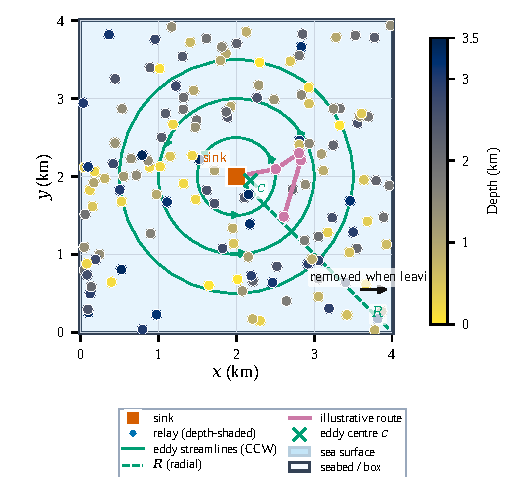
\includegraphics[width=\columnwidth]{fig4_deploy_top}
\caption{Deployment used in the evaluation (one placement, seed 20261801; top view, relays shaded by depth). The sink and the eddy centre coincide. The route and the eddy streamlines are illustrative.}
\label{fig:deploy}
\end{figure}

\emph{Scenarios.} Scenario~I is static. Scenario~II applies the eddy and Gauss--Markov flow of Section~\ref{sec:network} with a peak speed of 0.15~m/s, and Scenario~GM2 doubles the speed and the variability. A relay that leaves the volume is removed, which affects on average 22.3\% of the relays in II and 29.5\% in GM2. We had aimed at 15\% and report the measured fractions.

\emph{Intervals and estimators.} The packet cohort, the energy interval, and the control count are different intervals (Section~\ref{sec:metrics}): packets generated in $[900,14400)$~s, energy in $[900,14700]$~s, and control frames starting in $[0,14400]$~s. The primary estimator is the mean of run-level ratios, not the pooled ratio; a pooled sensitivity analysis for QELAR gives energy differences of $-181$, $-20$, and $-24$~mJ/bit against 120~s periodic in Scenarios I, II, and GM2, with the same sign pattern and bootstrap intervals that exclude zero only in Scenario~I.

\emph{Statistics.} MARV uses evaluation seeds 20261801--40 (40 per cell; the scalability and drift sweeps use the first ten) and QELAR uses 20261841--80. DA-HELLO configurations were locked on separate tuning seeds (20261114--23) that appear in no evaluation table. Comparisons are paired by seed. Non-inferiority is stated against an explicit margin: 0.5 percentage points (pp) for MARV, and 3~pp for QELAR, because the paired standard deviation of PDR differences on QELAR was 6--10~pp in the pilot, against below 1~pp on MARV. The QELAR margin was therefore chosen after the pilot and before the evaluation. Holm correction is applied within each pre-registered family of three scenarios; the intervals shown are unadjusted.

\subsection{Hosts, Arms, and Pre-Registered Statements}
\label{sec:arms}
\emph{Hosts.} MARV and QELAR are our re-implementations of the published rules. They carry state in data headers; for each we also run a labelled HELLO-only variant in which header attributes are stripped from data frames and only HELLO or beacon decodes write records. The variants are not reproductions of a published protocol.

\emph{Arms} (Table~\ref{tab:arms}). Every arm shares the host's routing logic and the same join announcement and 60~s sink beacon; only HELLO scheduling differs. B0 sends nothing after joining. Periodic arms send a jittered HELLO every $T$~s and receive one free full round at time zero, which favours them; $T=120$~s is the comparator in the pre-registered statements. The Trickle arm is tuned on MARV but uses the host's own timer defaults on QELAR, so the two Trickle results are not matched comparisons. The DA-HELLO configuration differs by host class and was locked on the tuning seeds.

\emph{Statements.} S1 (MARV HELLO-only): DA-HELLO is non-inferior to periodic 120~s in PDR at 0.5~pp and uses at least 50\% fewer control bytes. S1$'$: non-inferior in PDR, with fewer control bytes and lower energy per bit. S2 (MARV header): non-inferior to B0 at 0.5~pp with an energy change below 5\%. Q1, Q1$'$ (QELAR HELLO-only): as S1 and S1$'$ at 3~pp and at least 40\% fewer bytes. Q2: B0 is more than 5~pp below DA-HELLO. Q3 (QELAR header): non-inferior to the host alone at 3~pp with an energy change below 5\%.


\subsection{Results: HELLO-Only Hosts}
\label{sec:res-hello}
Fig.~\ref{fig:pareto} plots delivery against control overhead. Without HELLOs, both hosts collapse: B0 delivers 0.14 to 0.18 on MARV and 0.06 to 0.07 on QELAR, because no record is created after joining. Periodic HELLOs restore routing, but frequent ones hurt: on MARV, delivery in Scenario~I rises from 0.45 at 20~s (376~B/s) to 0.78 at 120~s (64~B/s), since HELLO traffic congests the shared channel, and the 5~s and 10~s periods saturate it (0.01 and 0.13 in Scenario~II, at 1275 and 647~B/s).

\begin{figure*}[!t]
\centering
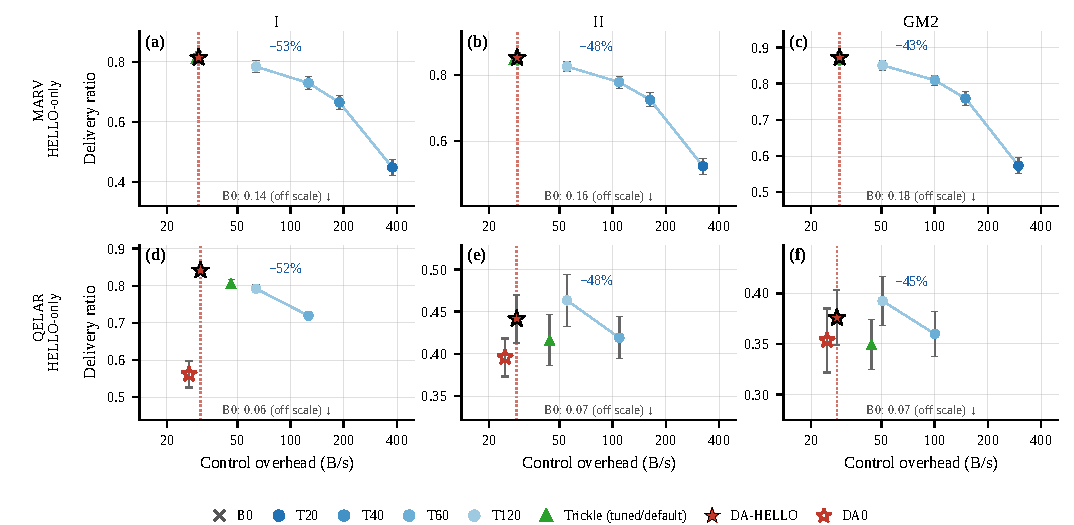
\includegraphics[width=\textwidth]{fig5_pareto}
\caption{Delivery versus control overhead on hosts whose state travels only in HELLOs (top: MARV variant; bottom: QELAR variant); $n=40$ seeds, bars are 95\% intervals. The no-HELLO value is off scale and printed in each panel. $y$-axes differ between panels. Percentages give the control bytes of DA-HELLO relative to periodic 120~s.}
\label{fig:pareto}
\end{figure*}

\begin{table*}[!t]
\caption{Pre-Registered Comparisons (MARV t103 Seeds $20261801$--$40$;
QELAR t109 Phase~2 Seeds $20261841$--$80$). $\Delta$ Is DA-HELLO Minus the
Named Reference; Intervals Are Paired Student-$t$ $95\%$.}
\label{tab:prereg}
\centering
\scriptsize
\setlength{\tabcolsep}{4pt}
\begin{tabular*}{\textwidth}{@{\extracolsep{\fill}}llrrr@{}}
\hline
Stmt & Sc & $\Delta$PDR [pp] & Rel.\ bytes & $\Delta E_{\mathrm{bit}}$ [mJ/bit] \\
\hline
\multicolumn{5}{l}{\emph{S1/S1$'$: MARV HELLO-only vs jittered T120}}\\
S1  & I   & $+3.01$ [$2.51$, $3.51$] & $-52.7\%$ & $-140$ [$-152$, $-128$] \\
    & II  & $+2.64$ [$1.99$, $3.29$] & $-47.6\%$ & $-121$ [$-132$, $-109$] \\
    & GM2 & $+2.15$ [$1.61$, $2.68$] & $-42.8\%$ & $-104$ [$-114$, $-95$] \\
\hline
\multicolumn{5}{l}{\emph{S2: MARV header vs B0}}\\
S2  & I   & $+0.60$ [$0.01$, $1.19$] & --- & rel $-0.1\%$ [$-0.9$, $+0.7$] \\
    & II  & $+0.64$ [$0.09$, $1.18$] & --- & rel $-0.0\%$ [$-0.7$, $+0.6$] \\
    & GM2 & $+0.44$ [$0.14$, $0.74$] & --- & rel $+0.4\%$ [$+0.1$, $+0.7$] \\
\hline
\multicolumn{5}{l}{\emph{Q1/Q1$'$: QELAR HELLO-only DA480 vs T120}}\\
Q1  & I   & $+4.95$ [$4.03$, $5.88$] & $-51.5\%$ & $-182$ [$-201$, $-163$] \\
    & II  & $-2.19$ [$-4.38$, $+0.00$] & $-48.1\%$ & $-30$ [$-145$, $+86$] \\
    & GM2 & $-1.67$ [$-3.65$, $+0.32$] & $-44.9\%$ & $+11$ [$-139$, $+161$] \\
\hline
\multicolumn{5}{l}{\emph{Q2: QELAR HELLO-only DA480 $-$ B0}}\\
Q2  & I   & $+78.2$ [$77.3$, $79.2$] & --- & B0 collapses \\
    & II  & $+37.2$ [$34.5$, $39.9$] & --- & \\
    & GM2 & $+30.5$ [$28.1$, $32.9$] & --- & \\
\hline
\multicolumn{5}{l}{\emph{Q3: QELAR header (FC off, $m{=}10$) vs alone}}\\
Q3  & I   & $+0.16$ [$-0.08$, $+0.40$] & --- & rel $E_{\mathrm{bit}}$ hi $+0.1\%$ \\
    & II  & $-0.41$ [$-2.42$, $+1.60$] & --- & rel $E_{\mathrm{bit}}$ hi $+4.3\%$ \\
    & GM2 & $+0.31$ [$-2.03$, $+2.65$] & --- & rel $E_{\mathrm{bit}}$ hi $+4.6\%$ \\
\hline
\end{tabular*}
\end{table*}


On MARV, DA-HELLO delivers 2.1 to 3.0~pp more than periodic 120~s, with 43 to 53\% fewer control bytes and 8 to 10\% lower energy per bit (Table~\ref{tab:prereg}); all intervals exclude zero. S1$'$ and the B0 contrast are met in every scenario, but S1 as written is met in Scenario~I only, because the byte saving falls to 47.6\% and 42.8\% in II and GM2, below the pre-registered 50\%. Against the tuned Trickle, DA-HELLO is within 0.25 to 0.60~pp of delivery, with a control rate within 4.5\% and 0.9 to 1.8\% lower energy per bit (the delivery interval excludes zero in II and GM2): it ties Trickle and does not beat it.

On QELAR the result is mixed. In Scenario~I, DA-HELLO gains 4.95~pp over periodic 120~s with 51.5\% fewer bytes and 13\% lower energy per bit. In II and GM2 it is 2.2 and 1.7~pp lower, with 48\% and 45\% fewer bytes. The lower bounds ($-4.4$ and $-3.7$~pp) fall below the 3~pp margin, so non-inferiority is not shown, and the energy difference has an interval that spans zero. Periodic 120~s therefore keeps a small delivery edge there at about twice the overhead. Against the other comparators DA-HELLO is clearly better: relative to the host's default Trickle it delivers 3.6, 2.5, and 2.7~pp more (the interval excludes zero in I and GM2) with 33 to 36\% fewer bytes and about 8\% lower energy per bit, and relative to periodic 60~s it uses 72 to 76\% fewer bytes and 14 to 28\% less energy per bit.

Table~\ref{tab:causes} shows where the HELLOs come from. First-contact replies account for most of them (5055 of about 8160 starts per run on MARV and 4679 of 8094 on QELAR in Scenario~II), the slow refresh for most of the rest, and membership and score-change requests together for under 160 per run.


\subsection{Results: Hosts With State in Data Headers}
\label{sec:res-header}
When data frames already carry the state, extra HELLOs add little and cost delivery (Fig.~\ref{fig:header}). On MARV, periodic HELLOs lose 37, 33, and 30~pp at 20~s and 4.3, 2.9, and 2.9~pp at 120~s relative to B0 in Scenarios I, II, and GM2, and the tuned Trickle loses 0.4 to 0.8~pp. DA-HELLO is slightly above B0 (+0.60, +0.64, and +0.44~pp), and its energy per bit differs from B0 by at most 0.42\%, so S2 is met; it also beats the tuned Trickle by 1.0 to 1.3~pp with about half the control bytes. We read this as no harm relative to doing nothing, not as a gain.

QELAR shows the same ordering with larger penalties: periodic 60~s loses 12.5, 13.7, and 14.2~pp, periodic 120~s loses 4.1, 6.3, and 7.1~pp, and the default Trickle loses 1.1, 8.0, and 11.6~pp. DA-HELLO with the first-contact reply on loses 0.2, 10.1, and 15.2~pp, and sends about 2900 first-contact HELLOs per run (Table~\ref{tab:causes}); with the reply off it is indistinguishable from the host alone (+0.16, $-0.41$, and +0.31~pp; Q3 is met) and sends about 12 membership HELLOs per run. We use the second configuration on QELAR's header regime. The two settings also differ in the rank margin, so this is a joint-configuration contrast, and we did not isolate why the reply is harmless on MARV but harmful on QELAR.

\begin{figure*}[!t]
\centering
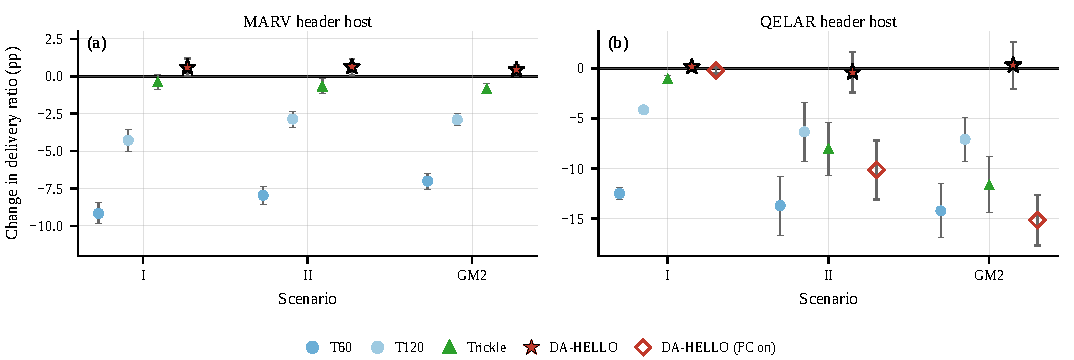
\includegraphics[width=\textwidth]{fig6_header}
\caption{Change in delivery relative to sending no HELLOs after joining (MARV) or to the host alone (QELAR), for hosts that carry state in data headers ($n=40$ per cell, paired 95\% intervals). The 20~s and 40~s MARV arms (losses of 12 to 37~pp) are omitted for scale. With first contact on, DA-HELLO on QELAR loses 10 to 15~pp in II and GM2.}
\label{fig:header}
\end{figure*}

\subsection{Components, Scalability, and Drift}
\label{sec:ablate}
\emph{Slow refresh.} On the MARV HELLO-only host, removing the 480~s refresh lowers delivery by 4.4, 1.8, and 1.3~pp in Scenarios I, II, and GM2 (all intervals exclude zero) and saves 5.6 to 9.1~B/s. A 240~s refresh lowers delivery by 0.8, 0.5, and 0.5~pp relative to 480~s and costs 10 to 14~B/s more (Fig.~\ref{fig:refresh}). On QELAR the same removal costs 28.0, 4.5, and 2.2~pp. The refresh therefore carries most of the delivery beyond first contact on HELLO-only hosts, and it is one reason why the configuration differs between regimes.

\emph{Score-change test.} The test raised between 12 and 160 host-state requests per run (Table~\ref{tab:causes}); on QELAR HELLO-only about 144 per run, roughly one per node, whereas the header configuration with the test off raised none. These are request counters, not transmissions, and we have no matched rank-on and rank-off comparison, so no performance benefit is attributed to the test or to the back-off.

\begin{figure}[!t]
\centering
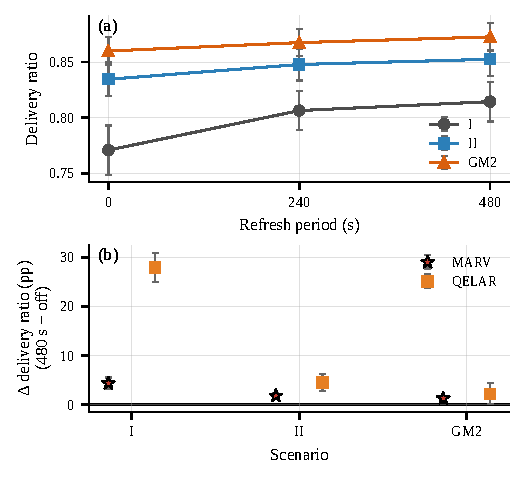
\includegraphics[width=\columnwidth]{fig7_refresh}
\caption{Slow-refresh ablation. (a) MARV HELLO-only delivery for refresh periods of 0, 240, and 480~s. (b) Paired gain of the 480~s refresh over no refresh, for MARV and QELAR ($n=40$, 95\% intervals).}
\label{fig:refresh}
\end{figure}

\begin{figure}[!t]
\centering
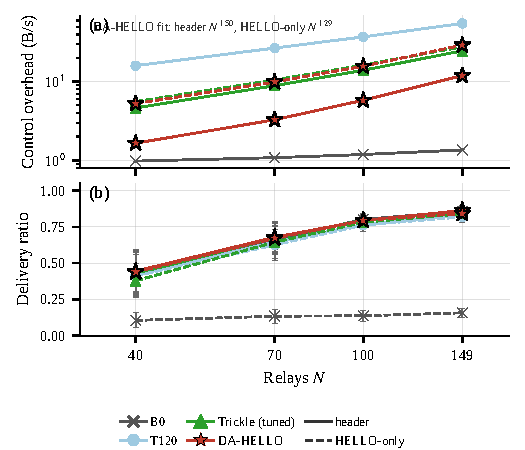
\includegraphics[width=\columnwidth]{fig8_scale}
\caption{Scalability in Scenario~II ($n=10$ seeds per point). Control overhead grows roughly as $N^{1.5}$ for DA-HELLO on the header host and $N^{1.3}$ on the HELLO-only host, below periodic 120~s and the tuned Trickle; delivery is low at 40 and 70 relays for all policies.}
\label{fig:scale}
\end{figure}

\emph{Scalability.} Fig.~\ref{fig:scale} varies the number of relays from 40 to 149 in Scenario~II (ten seeds per point). The overhead of DA-HELLO grows from 1.7 to 12.4~B/s on the header host and from 5.1 to 29.3~B/s on the HELLO-only host, which corresponds to power laws with exponents of about 1.5 and 1.3 in $N$. Periodic 120~s grows from 15 to 53~B/s and the tuned Trickle from 4.8 to 26.6~B/s (header host). Delivery is low for every policy at 40 and 70 relays (0.42 to 0.44 and 0.66 to 0.69 on the header host), owing to sparse connectivity and relay removal, and DA-HELLO stays within 0.1~pp of the best comparator at 100 relays. The energy per bit at 40 relays is not reported because one zero-delivery run has no defined value.


\emph{Drift speed.} Across mean speeds of 0.10, 0.15, 0.30, and 0.50~m/s (ten seeds), DA-HELLO delivers 0.839, 0.843, 0.859, and 0.867 on the HELLO-only host, against 0.813, 0.819, 0.835, and 0.843 for periodic 120~s and 0.832, 0.841, 0.852, and 0.861 for the tuned Trickle. On the header host it delivers 0.858, 0.863, 0.874, and 0.888, against 0.854, 0.858, 0.872, and 0.877 for B0.


\begin{table*}[!t]
\caption{DA-HELLO HELLO Starts by Cause in Scenario~II ($n=40$ Seed Means).
First-Contact Replies Dominate; Slow Refresh Accounts for Most of the
Remainder on HELLO-Only Hosts. Membership and Score-Change Requests
Together Stay Under 160 per Run.}
\label{tab:causes}
\centering
\scriptsize
\setlength{\tabcolsep}{5pt}
\begin{tabular*}{\textwidth}{@{\extracolsep{\fill}}lrrrrp{0.28\textwidth}@{}}
\hline
Host / arm & HELLO tx & FC reply & Refresh & Mem./rank & Notes \\
\hline
MARV HELLO-only & 8160 & 5055 & 2836$^{\mathrm{a}}$ & 44 & refresh$=$480\,s \\
QELAR HELLO-only & 8094 & 4679 & 3742 & 158 & mem 14, rank 144 \\
QELAR header (FC off) & --- & 0 & 0 & 14 & $\approx$12 membership \\
QELAR header (FC on) & --- & 2907 & 0 & 141 & descriptive \\
MARV header & 3155 & 2981 & 0$^{\mathrm{a}}$ & 24 & refresh$=$0 \\
\hline
\multicolumn{6}{l}{\footnotesize $^{\mathrm{a}}$MARV export codes slow-refresh and residual adaptive starts in \texttt{cause\_other}.}\\
\end{tabular*}
\end{table*}


\subsection{Pilot Runs on Further Hosts}
\label{sec:pilots}
Before the campaign, a host had to deliver at least 0.30 of its packets in Scenario~II without any HELLO scheduler on five tuning seeds. QELAR qualified (0.665 after aligning its candidate gate and previous-hop rule with its paper, up from 0.385). SAQR delivered 0.082 and LQARP 0.284 with an interval that spans the threshold, so neither was campaigned and we make no claim about DA-HELLO on them.

\subsection{Limitations and Disclosures}
\label{sec:limits}
The evidence supports a bounded statement. Where state travels only in HELLOs, DA-HELLO saves 43 to 53\% of the control bytes of periodic 120~s and delivers more on MARV; on QELAR it is competitive but not shown non-inferior in the drifting scenarios. Where state travels in headers, it matches doing nothing, and on QELAR only with first contact off. The configuration therefore differs by host class and is not self-adapting.

Several choices limit these results. Both hosts are our re-implementations, and 35 of 65 checklist rows of the host audit match the papers; the HELLO-only variants are constructed. Periodic arms receive a free first round, and B0 includes the sink beacon. Header bits that hosts add to data frames are not charged. The relay-removal fractions (22\% and 30\%) exceed the 15\% target and the removal rule affects the mobile scenarios. On QELAR, the pilot suggested +2.3 and +0.5~pp against periodic 120~s, but the evaluation gave $-2.2$ and $-1.7$~pp, and the 3~pp margin was set after the pilot. A matched first-contact and rank ablation, equalised start-up for the periodic arms, and a field-aware controller remain future work. The MARV raw run logs are no longer available, so MARV results rest on the retained exports. First-contact replies have a precedent in APU~\cite{chen2013apu}, and the void-triggered beacon in earlier void-handling work~\cite{ghoreyshi2017void}.

\FloatBarrier
\section{Conclusion}
\label{sec:conclusion}
This article proposed DA-HELLO, a HELLO scheduler for Q-learning
underwater routers that sends a HELLO on first contact with a new
neighbour, on a change of void status, and, optionally, after a long
silence. Evaluated on two re-implemented hosts, MARV and QELAR, with
state carried either in data headers or only in HELLOs, the results show
that the value of HELLO scheduling depends on how routing state is
disseminated. Where state travels only in HELLOs, DA-HELLO delivers
$2.2$ to $3.0$ percentage points more than a jittered $120\,\mathrm{s}$
periodic schedule on MARV with $43$ to $53\%$ fewer control bytes, and
saves $45$ to $52\%$ of the bytes on QELAR, although non-inferiority in
delivery was not established in its drifting scenarios. Where state
travels in data headers, DA-HELLO matches sending no HELLOs, whereas
periodic and Trickle schedules lose delivery; on QELAR this holds only
with the first-contact reply switched off. The score-change test showed
no demonstrated benefit. These conclusions rest on simulation of two
re-implemented routers. Future work will select the configuration from
the host's state carrier, test further trigger combinations, and
validate against field or trace-driven current data.


{\footnotesize
\bibliographystyle{IEEEtran}
\bibliography{refs}
}

\end{document}
